\chapter{Financialization} \label{chapter-financialization}
\epigraph{Financialization occurs when housing is treated as a commodity---a vehicle for wealth and investment---rather than a social good.}{Special UN Rapporteur on the right to adequate housing, Leilani Farha \cite{farhaReportFinancializationHousing2017}}

Financialization is the capture  of streams of surplus generated by society by financial actors.\footnote{There is a difference between investment in productive capital and investment in financial assets. The first contributes to total social output while the second is simply a transfer of ownership. The traditional distinction between capitalists and \glspl{rentier} pivots on this distinction. Capitalists invest in creating productive assets while rentiers live off the income generated by productive assets previously created. At the level of the economy as a whole, financialization can be seen as diverting savings from capitalist investment to rent-seeking investment. The economic system  that emerges as the process continues is sometimes described as rentier-capitalism \cite{christophersClassAssetsWork2021,  standingCorruptionCapitalismWhy2017}. In this thesis we are not concerned with the issues around the emergence of rentier capitalism, but mention it here to acknowledge the connection of this work to another literature.} 
It occurs at the micro-level through the development of instruments, and at the macro-level through larger system-level effects. Financialization is an inherently spatial phenomenon that should be analysed in an economic–geographic framework \cite{aalbersPotentialFinancialization2015}. This thesis is a study of the \gls{financialization} of the urban housing market, and particularly the system level effects of financialization on distribution and urban productivity. 

% {\color{red}
% MOVED FROM MODEL CHAPTER
\subsection{Financialization} 
%Our goal is to look at the relationship between urban production/labour markets, agglomeration, and land/housing markets. To explore this relationship we build a simplified model of a \gls{housing market}.% CALL IT LAND, PROPERTY, OR HOUSING MARKET? % - it is the housing use, combined with location we're interested in. % we introduce a \gls{land market}.% Agents purchase homes though a housing market. 

% In cities, housing is exchanged on a market. The product is properties, whether they're apartments, or land with the buildings on it. Properties have features including building size, style, quality, and location  that affect their desirability. %the buildings have a particular size and characteristics. %with various buildings and features. %properties on them. 
%Location also matters, %Land value  is affected by various elements
%including proximity to natural features like lakes and mountains, and human-built features like communities, and businesses, as well a developments and additions on the property itself. 
%Thereal market invovles  a set of agents who engage directly like buyers, sellers, renters, investors, and developers; as well as others who shape the market indirectly, including policymakers, activists, and neighbourhood and industry groups.
%The actors work within the context of a layer of policy, institutions, and rules. For example financial institutions offer debt, zoning allows certain uses and disallows others, and tax rules shape financial returns.

% and charges taxes and fees which are factored into the cost structure.
% shapes the land value.
% Our simulation model extracts % #E IS THIS A TECHNICAL TERM? i DON'T KNOW WHAT IT MEANS? yOU USE THESE TOGETHER. IF ITS STANDARD USAGE IGNORE THIS COMMENT
% these features to explore a core set of questions about financialization in land markets, in a way that's extensible to study a broad range of questions about real/particular markets in particular places.
% We study \gls{financialization} in a simplified market model, integrating
% In the simplified market model, %  owners sell when the retire.
% we integrate the % spatially explicit property market
% our urban production model  into a spatially explicit {housing market} with financial investment. %\gls{financialized} investment.

%Urban productivity drives land values through the housing market. Where there is a strong labour market, residents have a greater willingness to pay for housing \cite{GET_productivity_price_link} %ELABORATE. 
% Other factors also shape prices, including \gls{amenity}.

% *** In the model, rising \gls{population} and \gls{productivity} generate an economic value for land, that's derived from its proximity to the \gls{urban center}. 

% Use of a unit of land in each cycle is valued at the wage premium net of transportation costs. 
 % A worker, located at a distance $d$ from work, paying as much as $w- {dc}$ in rent, would still choose to work.

%\subsection{The microeconomics of  financialization} \label{section-micro}

Financialization happens at this microeconomic level, where individual decisions are made and real assets are bought by individuals and institutions. 
Properties have features including building size, style, quality, and location that affect their desirability. 
Agents exchange properties on a market,  
% Individual home-buyers are buying a stream of housing services and possible capital gains. Institutional buyers are buying 
and the return on housing as an investment is part of all agent's decision process. 
Private homeowners live in the properties they purchase, so when they purchase a property, they are buying both a stream of housing services and potential capital gains. %When a home is bought to live in, the potential buyer %makes a similar calculation, perhaps with a 
They may place particular emphasis on the value of the stream of housing services that matter to them individually. When home prices rise rapidly, speculative gains may become the dominant concern of home buyers. 
Investors, on the other hand, buy a stream of net rents plus speculative gains.
Each agent has their own interest rates, discount rates, mortgage share, information, and expectations, so individual bids can differ. 
%In the process, the real asset takes on an additional and separate aspect as financial object that can be bought and sold.  % The feature that matters most to investors is the  \gls{rate of return} that  an asset offers. 


% For any level of risk and liquidity, an investor will choose to purchase the asset with the highest expected rate of return. 
% To model the investment decision  we calculate the \gls{rate of return} on each property taking into account the rental revenue, the potential capital gain, the investors' costs of capital, incomes, and assets. The analysis will show the incentive structure driving the  financialization of the housing market. We do this in detail in Appendix~\ref{appendix-bid-price} 
% The model must  allow for bidding and speculative investment but also must reflect the underlying economic value driven by urban productivity. To calculate the \gls{rate of return} we, therefore, need to define the relevant variables, and make some distinctions among different notions of rent and price %, including a variety of prices perceived prices  bid price3s

% }

We are concerned with  effects of financialization at the level of the urban system, but to understand those effects, one must first understand the whole process, beginning with what financialization is, and the financial tools that form the building blocks of financialization. 
% Financialization is occurring if there is an 
%In this thesis, we explore the systemic effects of financialization on urban productivity. In this chapter, 
We introduce financialization as an \gls{emergent} phenomenon, using an analogy with digitization, look at financial instruments such as stocks, mortgages, and Real Estate Investment Trusts, then discuss potential systems-level effects of financialization.\footnote{On the recent history of the term, Aalbers observes that, ``[t]he concept of financialization has been used for a couple of decades by a small group of academics and other intellectuals, for example in the circle surrounding the Marxist Monthly Review (e.g. Sweezy, 1995), but it is only since the global financial crisis that started in 2007, that the term has acquired the status of a popular concept in a range of literatures spanning the different social sciences and the humanities.'' \cite{aalbersVariegatedFinancializationHousing2017}}


Financialization can be measured as an increase in the stock of financial assets associated with a stock of some set of real assets. This is why the term is often used as a collective noun for the growth in the number and/or size of  transactions, creating or transferring financial assets to financialized ownership \cite{GET_financialization-numberOfTransactions}. % These transactions typically occur through a \gls{market}.  
% While there is no clear point in time when global financialization began, 
% In 2013, wrote that 
It is this sense  Tomaskovic-Devey and Lin use when they wrote in 2013 ``[t]he U.S. is now a financialized economy, where the financial sector and its priorities have become increasingly dominant in all aspects of the economy'' \cite{tomaskovic-deveyFinancializationCausesInequality2013}. Christophers argued in 2015 that approximately 40\% of the economy was financialized. Aalbers, however, points out that, since many financialized firms are classified as part of the real economy, 40\% may be  a substantial underestimate. \cite{aalbersPotentialFinancialization2015}.

While there is not a single point at which financialization began, its dominance has arguably consolidated through the expansion of financial capitalism during the period from 1970 to present, in which debt-to-equity ratios increased and financial services accounted for an increasing share of national income relative to other sectors. Thomson and Dutta, \cite{thomsonFinancialisationPrimer2018}, suggest that August 15$^{th}$, 1971, when American President Richard Nixon announced that the United States would unpeg its currency from gold, marks a turning point in the financialization of the economy. This accelerated growth in global liquidity and prompted a surge of financial liberalisation and deregulation and undermined the Bretton Woods System. Synthetic derivatives were created soon after: The Chicago Mercantile Exchange launched futures contracts written on financial instruments the following year and the Chicago Board of Trade introduced the first interest rate future contracts three years later. Arbitrage, options trading, and various other activities grew exponentially. By 2011, the over-the-counter (OTC) and exchange-traded derivatives market amounted to almost \$800 trillion. Wijburg et al \cite{wijburgFinancialisationRentalHousing2018} argue that the financialization of housing markets in Germany, Spain, the US and elsewhere largely took place in the seven years before the global financial crisis  of 2007. 


Financialization is a global phenomena. Markets in different jurisdictions are regulated differently so the effects vary across countries. There is, however, a ‘common trajectory’ \cite{hayCommonTrajectoriesVariable2004}\cite{aalbersConversationLandRent2018} in which local economies evolve from different starting points subject to similar economic pressures.  In this thesis we refer most often to housing market data for Canada and Ontario. In our discussion we move between general historical trends and we draw on American financial history because of its significance on the global financial stage, but use specific and numbers from Canada. 

% Recently , particularly since the 2008 housing crisis, the financialization of housing has been a big piece of this 
Recently, financialized ownership of housing has increased while homeownership rates have declined \cite{statisticscanadaBuyRentHousing2022}.
70\% of new condo units in Ontario are purchased by investors \cite{GET_ontario_condo_ownership}.  About a third of the value of  owner-occupied homes in Canada is held as mortgages. In other words, about a third of the net land rents associated with owners-occupied housing accrues to the financial sector. Since 66\% of Canadian homes are owner-occupied,  5/9 of the Canadian housing stock is owned as financial assets \cite{nemtinFinancializationHousingSocial2021}. % blackstone. CHECK


\section{Financialization is a process like digitization}
Financialization is an emergent process, something % ?? SOMETHING?  that takes place through a series of steps across different scales/levels??? <<< EDIT THIS
driven by individual micro level actions, that interact to have much larger, potentially unexpected effects at a system level. We can think about it as something like the process of \gls{digitization}. 
Through the late 20$^{th}$ century to the present, activities have increasingly shifted from being the analog operations of material, mechanical systems  to digital content manipulated digitally on micro-electronic devices. 

The digital revolution happens at different scales. At the micro level there is the development of technologies, such as transistors, integrated circuits, and the wide array of products built from them including mainframe computers, laptops, and smartphones.  

At the macro level, digitization represents a fundamental system change, reducing transactions and transformation costs, and creating a vast array of digital products that are almost costless to reproduce and distribute. Digitization created huge new industries like video streaming, electronic monies, and coding. It has also vastly expanded other industries, %like streaming and delivery systems,
cut transaction costs, expanded consumer choice, %as services like Amazon become so successfully, 
and hugely increased the dissemination of intellectual content though electronic publishing and in movie and music creation.   
%  change the mind society to Google vs to think, come to talk with each other. communications, algorithms, inteligences, categories, minds

Digitization was not and is not a planned process, but rather the result of millions of individual decisions, each in pursuit of specific, local, individual goals, and ideas about what is happening in the system. The pursuit of these goals supported the development of  new supply chains and institutions. As with financialization, the cumulative effect was a systems level change with wide ranging effects.  Like  financialization, digitization is an emergent and transformative feature of the economy.

\section{Instruments of financialization }
To financialize something requires a \gls{financial instrument}, with two primary features: first that it represents something of value, and second, that it can be bought and sold as an investment. These instruments represent rights to packages of surplus value that can be redeemed in the future, converting the product of real-world activities into financial assets that can be traded easily. 

At the micro level, therefore, financialization is achieved through the development of legal and financial instruments that allow for exchange. These instruments become the building blocks enabling the process of financialization. There are numerous kinds of legal and financial instruments.
% In Financialization, legal and financial instruments are like the products that enabled the digitization of a increasingly wide range of activities. %that make digitization possible:  %, and financial instruments have been central to the housing system for a long time. 
% in the housing market and in the broader financial system. % 
%Examples of financialization outside the housing system include stocks and stock markets. 

The most well-known and quintessential financial instrument, stocks, form the basis for the modern stock market, and perfectly illustrate the core features of financial instruments. % and their systemic effects. 
Stocks originated as a financing mechanism for the \gls{joint-stock company}, and act as a %are an important 
mechanism for channeling investment into productive activity. They have their roots in the European colonial period and are among the most important financial instruments in the modern economy. %capitalist economy.  

% The development of 
The joint-stock company %fundamentally just a financial instrument  
facilitates the pooling of investor funds with specific legal protections. It provides a powerful example of a financial instrument that ultimately transformed the economy. There are records of joint-stock companies being formed in Europe as early as the 13$^{th}$ century. They multiplied beginning in the 16$^{th}$ century. The Virginia joint-stock company was chartered in 1607, not only for the purpose of creating new trading opportunities, but also for the purpose of establishing colonies in the acquired lands of North America.  It was the Virginia Company's London branch that established the first permanent English settlement in the New World. The East India Company was founded in 1600 to trade in the Indian Ocean region, initially with the East Indies and later with East Asia. The company funded armies, seized control of large parts of the Indian subcontinent, and colonised parts of Southeast Asia and Hong Kong. At its peak, the company was the largest corporation in the world. 

The development the joint-stock company, a financial tool, enabled both political takeover and a vast expansion of global markets, which in turn helped drive economic growth and technical innovation, changed wealth flow at a global level, and changed ecosystems, power structures, cultural practices, and even what languages people spoke. The financial instrument enabled a shift in the flow resources, and that shift had a much broader shift in systems at a global level. % language use%and even changes in cultural practices, language use, education, and more. 

%With an excess landless population to serve as workers, and motivated, adventurous, or devout investors, the joint-stock company became the vehicle by which England finally settled the Western Hemisphere. 
% AUTHOR	ushistory.org
% TITLE OF PAGE	Joint-Stock Companies
% TITLE OF PROGRAM	U.S. History Online Textbook
% URL OF PAGE	//www.ushistory.org/us/2b.asp
% DATE OF ACCESS	Wednesday, March 29, 2023
% COPYRIGHT	2023



%Stock markets are a primary means of mobilizing long-term savings and investment for fixed capital formation \cite{azfarMarketMobilizedCapital2003}. 
Stock markets make it possible- the market in stocks- manage risks, but can also allow emergent phenomena like bubbles and crashes.
Originally a tool to allow a group of investors to pool their money, take on large projects, and to share risks, stocks themselves rapidly became objects of trade and speculation with the formation of  the first stock market in Amsterdam in 1611. Stock markets allow stockholders to buy and sell existing stocks, but they also allow promoters  to sell shares in new companies. There is disagreement about about how much  stock investment is simply speculation and how much creates productive real assets.\footnote{Mork et al. identify four theories that attempt to explain the correlation between stock returns and subsequent investment \cite{morckStockMarketInvestment1990}. \begin{quotation}The first says that the stock market is a passive predictor of future activity that managers do not rely on to make investment decisions. The second theory says that, in making investment decisions, managers rely on the stock market as a source of information, which may or may not be correct about future fundamentals. The third theory, which is perhaps the most common view of the stock markets influence, says that the stock market affects investment through its influence on the cost of funds and external financing. Finally, the fourth theory says that the stock market exerts pressure on investment quite aside from its informational and financing role, because managers have to cater to investors' opinions in order to protect their livelihood. For example, a low stock price may increase the probability of a takeover or a forced removal of top management. If the market is pessimistic about the firm's profitability, top management may be deterred from investing heavily by the prospect of further erosion in the stock price.\end{quotation} None of the point to a direct connection between stock market investment and real investment.} % Share prices on the stock market are not tightly tied to the productivity of the company they represent, illustrating how the financial instrument can diverge from the real asset, and making it clear that the financial instrument is something different from the real asset. % Stock transactions can also be speculative. Most stock transactions are speculative in nature 
% Financial instruments can be combined and new types of instruments built on top of them. For example, mutual funds, which pool more risky stocks, in an effort to offer more reliable returns, are a financial instrument built on top of the stock market.
% Over time these developments have produced substantial systems-level effects. \cite{hayCommonTrajectoriesVariable2004}

% it makes it possible to movilize capital, for speculative bubbles to form, for distant markets to become more tightly coupled and interelated in their business cycles.

%Had armies. Changed the language, economic flow, concentration of wealth

% Instruments are built on top of thiem like mutual funds which purchase stocks and buld a portfolio, so that investors can spread their risks adcross multiple companies.  There are also whole structures of speculative instruments, that are essentially bets on the performance of other instruments. Deriviatives don't require actually purchasing stocks---they bets on the performance derived from other aspects of the economy. There are now vastly more derivatives in the economy than real assets. These bets may offer information about value, or speculation. They also may add a range of systemic risks, as there is this edifice of wealth that hangs on financial performance of a relativley small number of companies that produce something someone might want. %-profits not production


\subsection{Mortgages}
One foundational financial instrument that changed the structure of the housing market is the mortgage. 
Mortgages began as  a financial instrument that enabled individuals to make purchases larger than their saving - mainly  purchase properties.   They have become a financial asset that can be bought and sold as property in themselves. This allows investors to purchase mortgages as assets when they think the return on  return  is higher that the return on other assets.  When mortgages become an easily exchanged financial asset, they begin to serve as a channel for money to move into the housing market, not to produce additional housing for the market, but to capture value from the market. The two uses of mortgages demonstrate two aspects of financial instruments.  

Mortgages have always allowed lenders to participate in housing purchases in the present in exchange for a future flow of payments. The mortgage does not by itself create housing, but it enables a prospective buyer to become the nominal owner of an asset, in this case a house, that produces a stream of benefits such as a place to live, proximity to work, and proximity to services, natural features, or other amenities. The value of housing is set by the market to factor in not just the features of the home itself, but the locational value of the property based on the stream of benefits provided. 

Because the value of the stream of benefits from secure housing near a source of income generally exceeds a buyer's current assets, mortgages were created to  enables the transfer of ownership by making it possible to transfer the rights to a substantial fraction of the future income of the buyer or mortgagee to the mortgage holder. In effect, the mortgage holder remains the property owner until the terms of the mortgage are fulfilled.  If the mortgagee fails to make those payments, the mortgage holder will repossess the asset. The security provided by this instrument ``de-risks'' the transaction, making it safer and therefore easier to achieve the mutual benefits of the sale. 

The additional step of making these mortgages tradable on a market is required to create a financialized market. Originally mortgages were an arrangement between just the buyer and the seller, but in the 1870s in the USA, insurance companies stepped into these transactions, paying off the seller and then collecting the principle and interest payments on behalf of the bank's shareholders. This innovation was an example of financialization in that it made it possible for financial actors, in this case, individual insurance companies, to profit by providing money to buyers. It also had systemic effects, making homeownership accessible for more people. When mortgage lending was regulated and insured  by the American government during and after the great depression it facilitated a further massive increase in home ownership in the USA and contributed to the post-war construction boom and the suburbanization of American cities. 

The housing market was thus initially financialized by the market for insurance-backed mortgages, but these mortgages were still agreements between individual lenders and buyers. When financial institutions later developed markets that let them buy and sell bundles of mortgages among themselves, we say the mortgage market itself was financialized. This added % ADD DATE
a secondary market for the promises to pay that every mortgage represents on top of the market for housing financed by mortgage-type loans.
%

The addition of new levels of financialization do not (necessarily??) affect the functioning of the lower-level financial instruments. Buying and selling packages of mortgages does not directly affect the condition of the individual mortgages---they simply add a new product for investors or banks to buy and sell. 

Introducing such  markets can have an effect at another level, however. The new market in bundled mortgages, for example, was thought to further reduce the risk for lenders, but between 2007 and 2010 in the USA the sub-prime mortgage crisis destabilized the financial institutions that were playing this new market.\footnote{Arguably, that crisis resulted from overselling risky and predatory mortgages by lenders with more money to lend than the market could absorb. Eager investors seeking higher or more secure returns were willing  to buy bundles of  mortgages that were in theory de-risked. Pooling uncorrelated individual risk, as the insurance industry does, produces lower overall risk. (The instruments that enabled the speculative bubble were mortgage-backed securities (MBSes) and collateralized debt obligations (CDOs).) Pooling does not reduce systemic risk, however. As it turned out, the mortgage default rate rose, lenders' liquidity fell, mortgage rates were pushed up, defaults increased, and the market for the new instruments collapsed, taking down major financial institutions, providing a cautionary tale about potential costs of financialization. Analysis of that case may provide a cautionary tale about the the potential risks of financialization.} 
This is an example of a cross-scale effect of the type that we are exploring in this thesis.  

Note that mortgages are clearly, financial instruments, but not all financial instruments are instruments of financialization. Ownership of the promises to pay can be increasingly financialized---captures the value of the stream of house payments, can be exchanged, and is freely traded in financial markets. If debt is central, the share of the financialized ownership.
If financialization is the increase in the share of surpluses claimed by investors, and financialized owners, mortgages can do that, allowing some to invest in and claim a disproportinate share of future urban productivity. They may also function to transfer ownership of property to at least some individual community members, perhaps transferring the asset from the financial interests which funded development, to local distributed ownership, by community members primarily concerned with the use value of living in the house. This not only localizes distributes ownership of the stream of surpluses, and potentially acts to decouple it from larger financial interests and cycles. 
% ADD BACK {Financialization is not good or bad in itself}. %- asses by its resilience property, coupling in the system, it mobilized capital. Investors have many features- can it promise, who carries the risk in case of failure. 


\subsubsection{Investment trusts}
% allow vastly more inflow of finance into housing markets. 





The process of financialization of the housing market has also involved the development of new financial instruments, that are specifically suited to financialized ownership of housing. An example of a financial instrument designed specifically to support rent extraction and which increases the degree of financialization of the housing supply is the Real Estate Investment Trust (\gls{REIT}). 

A REIT is a company that owns, operates, or finances income-generating real estate and distribute the income to shareholders. While the company itself is an management system, the shares are are simply financial assets that are that are sold to individuals and organizations that want to share in real estate revenues and capital gains. 

Developed in the USA  in 1960 (as an amendment to the Cigar Excise Tax Extension!) and introduced in Canada in 1993 \cite{GET_REITsDevelopedDates}, REITs are similar to mutual funds in that they make it possible for an individual, often small investors to earn dividends from real estate investments without having to buy, manage, or finance any properties themselves.They can offer high rates of return because they actively push up rents using several devices \cite{GET-Martine-August, farhaReportFinancializationHousing2017}. Like mortgages REITS are financial instruments, but they directly expand financialization of the housing market by buying housing on behalf of financial actors. 

REITs have become increasingly popular in recent years. There are other large owners of residential real estate such as life insurance companies and pension plans that behave similarly, but REITs are a relatively new financial instrument which is expanding rapidly and attracting political attention for their effect on housing markets.  % REITs that develop new properties generally don't sell the properties they construct. 
An S\&P-Dow Jones research bulletin reported that over the 25 years to 2017, REITs outperformed stocks, bonds, and commodities \cite{GET-Dow-Jones-research-bulletin}. Because they have outperformed competing investments they have attracted  capital from other uses, particularly during the recent period of low interest rates.\footnote{There are questions about preferential tax treatment, and whether some REITs are essentially inappropriately sheltered real-estate corporations.} For the purpose of this thesis, REITs are simply one of the mechanisms for the financialization of housing.

% IMPORTANT - ADD BACK! REITs invest in properties with the aim of claiming rents, and often aim to increase rents, either by investing in upgrading apartments, transferring costs to tenants, or displacing people. % Martine August has interviewed tenants who have had larger investor purchase their property then refuse to do things like service toilets. %Deep pockets and able to manage legal feels.
% \textbf{fix toilets}, - want to bid up, vs renters with power to keep rents down- need a mix - if hunan capitla - competinf for the frontier speculatively. pay people to burry money in their backyards \dots role of interest rates making this more attractive. 


% \begin{figure}
% \centering
% 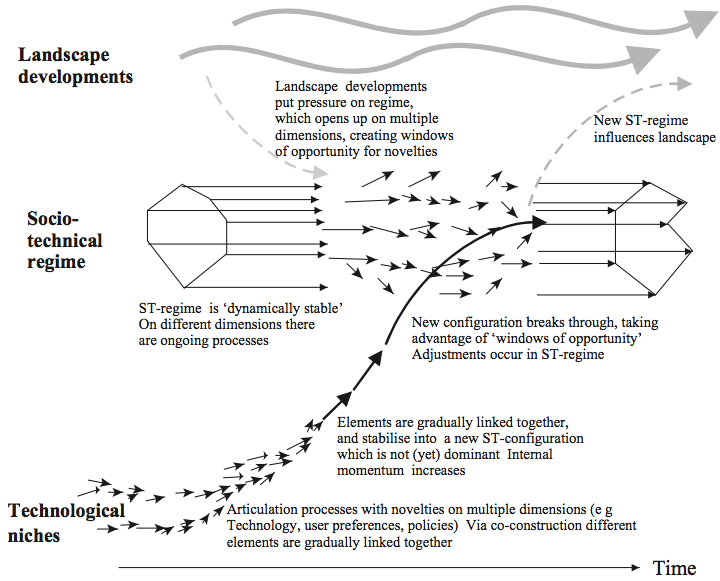
\includegraphics[scale=.60]{fig/transitions.png}
% \caption{Transitions occur across scales (Source Geels 2002).}
% \label{fig-transitions}
% \end{figure}

\section{Systems change}
% \section{Financialization as an emergent property}

%A third aspect of the word financialization is these system level effects of financialization.

% We have called attention in this section to the development of several important financial instruments---stocks, stock markets, derivatives, mortgages, and REITs---with the intention of  disentangling the concept of financial instruments from the term ``financialization.'' The development of instruments facilitates the process of financialization, but is not, in itself, financialization.

%We have called attention in this section to the development of several important financial instruments---stocks, stock markets, derivatives, mortgages, and REITs---with the intention of  disentangling the concept of financial instruments from the term ``financialization.'' The development of instruments facilitates the process of financialization. It is not, in itself, financialization, however.
Like digitiazation, financialization also has systems level effects. Thomas Palley describes financialization as ``a process whereby financial markets, financial institutions, and financial elites gain greater influence over economic policy and economic outcomes. As we've seen through the examples in this chapter, Financialization transforms the functioning of economic systems at both the macro and micro levels'' \cite{palleyFinancializationWhatIt2007}. 

% There are different kinds of systemic effects of this kind of increasing control and coupling could have/appear to have ELABORATE
There are many systems effects. ADD MORE %Jammison goes further and argues that the material and economic relations can actually structure our relation to society and ourselves, and even the ability to solve problems (e.g. methaprical structures limit ability to deal with societal crises like climate change).
We focus on the distributional effects, and hysteresis.

To illustrate the potential for systemic shifts, we describe some of the system level effects of the widespread adoption of instruments for the financialization of housing introduced earlier, mortgages and REITs. 
% This process of financialization also has profound impact at systems level. 
% And the word financialization, at the macro level, refers to this set of impacts.
% THOUGHT TO LOWER RISK  %DID THE CRISIS SHOW IT DIDN'T?
% The instruments and share are not neutral tools. They have the potential to have a profound effect at the level of the system.

Mortgages can influence the system in a number of ways. ADD %When we consider urban housing, 
A mortgage is the right to future income generated by capital, labour, and the city itself through the agglomeration effects that drive productivity. It is an instrument that indirectly captures a share of the urban rents. As productivity rises, wages rise, rents rise, property prices rise and mortgages rise, so the anticipated value of the future rents shapes the value of the property value. %The result is that there is a rent available that owners can claim. % \textbf{The effect is ADD}

REITs also have system level effects. %are not a neutral tool for saving either. 
According to a paper \cite{wangAnalyzeImpactREITs2021} on REITS in the Irish housing market, ``REIT successfully reconnected the international financial market and the Irish real estate market.'' In other words, in Ireland, REITs have made it easier for international capital to buy Irish land. The entry of outside and footloose capital has had an effect on the resident population:  ``the large-scale acquisition of Irish real estate by REITs and other real estate buyers has also caused some new problems. First, the active management of assets by REITs and other investors has led to a rapid increase in rents.''\footnote{In  IMF working paper ``Capital Account Liberalization and Inequality'' \cite{furceriCapitalAccountLiberalization2015}  Furceri and Loungani reported that that for 149 countries from 1970 to 2010, ``after countries take steps to open their capital account, an increase in inequality in incomes within countries follows.'' The observation is consistent with our argument  that domestic \gls{rent-seeking} in housing markets will increase inequality.}  

There is evidence that REITs affect real estate markets in other ways. Bat et al.  \cite{batRolePublicREITs2022} report that  ``they are actually financial actors that aggressively buy up property assets and manage them to extract wealth at taxpayers' expense.'' and ``they have expanded the pool of capital available for transactions that monetize real property and turn it into tradable assets---financial widgets with little or no connection to the real purpose of the productive enterprises that occupy the properties they own.''

\section{Summary} 
Financialization of the housing market is the increasing control of the stock of urban land and housing by investors in order to capture the scarcity rent generated by the people of the city, and the system level effects of that increasing control.  In this chapter, we've discussed what this means at the level of finance and the development of particular financial and legal instruments, at the micro-economic level as these instruments are taken up, and we've introduced some of the broader macro system effects of this process of financialization. The rest of the dissertation is a further exploration of the systemic effects of this process. 

% \section{Notes}
% Marriana Mazucatto \cite{mazzucatoValueEverythingMaking2018}
%https://www.ohchr.org/en/special-procedures/sr-housing/financialization-housing
%https://www.tni.org/en/publication/financialisation-a-primer#Q5

% Financialization has become a major theme in Canadian discussions of what is increasingly seen as \dots
%the increasing share of housing owned by investors, 
% Individuals develop ideas about how the society is transforming


% This phenomenon operates on multiple scales. % including the development of individual legal and financial instruments, the process by which actors capture a larger share of the surplus, and the larger system level effects of that process. % and their adoption and scaling, to larger systemic effects of the process oto facilitate the claiming of rents. %/across scales.
% At the microeconomic level, it is a.  %At a macro level it refers to the effect on the system itself of the new instruments and the increase in the type of transaction that they make possible.

% They are not unprodictive, and they can mobilize resources for good things. Investors can be good/productive. 
% SCALING OUT VS SCALING UP \dots
% % As in digitization, financialization has three elements, there are the individual financial and legal instruments for claiming rents, these are the inventions or technologies.
 % In finance, it is a term for the  (is there a better linking word than 'involves'?
% Financialization involves this process of developing the legal instruments that facilitate financial transaction.
% There's the process by which a particular innovation is taken up and adopted, and then there are the system level effects. %, the subject of this work. 

% Arguably there are no conscious forces promoting financialization. There are conscious forces at the systems level coming to understand and seek alternatives. This work and the broader 
% +++++++++++++++++++++++++++++
% of work on financialization for instance are individual pieces of work engaged in  the larger shift to f the system. The line between them 



% intention and financialization.
% wanting new yellow calculators can derive
% rewardign to claim so there is a lot of intent
% persuing own goals.
% in the formal economic model this tends to be in the dirrection of economic rationality, for the sake of generality, it can be any onw goals - whether minimizing risk, preserving wealth for kids, maximizing personal or family development, being surouded by colours or patterns that stimulate a chemical response, free time, minimizing mental effort, following shiny things, seeking truth, being influenced. Formallyt we don't wpecify what their own interests are.  we draw an arbitrary boundary within a particular model of the local process \dots 






% since nobody wins in the new world as a whole. IT is highly sub-optimal. actively promote a particular profitable instrument.
% Regan, Friendman candlens. - consciosu theoretical shifts towards this.

% A world wehre the---the process is the capture, with or without intent. The process is defined at the micro level. The macro level results are inherent in that process. Our whole appraoch is centered on talking about the macro level phenomena, while holding rigorous grounding in the micro level of individual reactions, actions, motivations - it becomes a structure that can be filled out on many levels. 
% - it both drives and is driven by macro level, emergent effects as well as the micro level phenomena \dots - system level effects, attemtps to theoreise it, effects that are analagous to - mind has a mind- - attempts to theorize that respond to the emergent level phenomena, attempts to understand, articulate and repsond, what we'd understand---are micro level actions in response to formulation, to theories and ideas about the macro-level phenomena.

% ADD BACK Each act in the process of financialization is directed toward the capture of the streams of the surplus created by society. Each is implemented  through particular legal or financial structures, which is to say through social technologies. Success leads to wider adoption of those technologies or rules. The system-level impacts of the growing use of these technologies is the  subject of this thesis. In particular, this thesis focuses on the potential macro effects of financial capital capturing spatial urban rents. 

% The opportunity to capture a part of the urban surplus leads to the creation of new financial instruments and ultimately may change the structure of the urban housing system 

% MOVE TO SYSTEMS IMPACT. There is an act that produces a surplus that individuals persuel. bEcause there is a flow of surplus, there is the finance to develop whole instituteions, whole professions around doin git.  - EMPHASIS IS THAT - it is an emergent property. visible at certain thresholds, hard to reversible after certain thresholds. A financialized system has emmerged, not been planned but emmerged. (no plot but many plots)

%People are involved at every stage, they create strucutres, the help adoption , by particualr actors, people in the legal or financial sector, sellers, real estat agents etc.  - and reacting exploitjng to ti

% INTRO DEFN ALIGHN ''Financialization of the housing market refers to the growth in the share of the housing stock controlled by financial institutions and investors and the overall effect this has on the outcomes of the system \cite{farhaReportFinancializationHousing2017, hansenFinanceCapitalismFinancialization2014}. 


% ''Financialization is the process of capturing streams of surplus generated by society. The agglomeration processes that creates cities produces a growing stream of surplus and some of it appears as locational rents. Fianncialization of the housing market is the process capturing a larger share of urban locational rents. 

% Financialization is a process of capturing rents. It can be understood as a social innovation \dots

 
% There are three components

% there's the invention, the adoption,and the set of systems impacts.


% The analogy with digitization is worth extending.
% Can be understood as analagous to digitization. 
% ***E %tHIS PARAGRAPH IS AWKWARD TO READ
% In the development of information technology, there are particular technologies, which are developed and refined. For instance the transistor. Basically a logic switch. There is nothing new about a switch but they can be made so small they can be combined together into devices, calculators and eventually mainframe computers that research institutes purchased. The one at the Davis Center filled a whole floor, people wrote whole programs
% and there's this painstaiking phase, teaching the computer what people knew.
% The series of devices, mainframes, then personal computers, then phones miniaturization made computing ubiquitous.

% ADD BACK As with digitization of the economy, any single act, the adoption of one computer, had little effect. People find an action that can be profitable, see a local opportunity, replace one mechanical calculator with a digital calculator, but the collective effect was large.  There are many system level impacts: banks lay off half their workers, the devices can talk to each other, connect vast data sets, etc. 
% may be large
% At the individual action It's morally neutral as well.
%individuals can create what would have taken a publication studio, a film studio, 3D print, can bank from home.  \dots system level they can talk phases \dots

% For finncialization aim to capture flows of the surplus. legal and financial isntruments to do it. banks-- investmetn fuels it \dots

